% !TEX root = ../../report.tex

\section{Mathematische Verfahren}

\subsection{Verzerrung von Bildern}

\subsection{Blending}
Blending ist Verfahren welches es ermöglicht überlappende Teilbereiche von zwei Objekten zu definieren.
Im einfachsten Fall - so wie auch in unserem Projekt, kommt das Alpha-Blending zum Einsatz.
Dieses sorgt dafür, das transparente Bereiche zweier Objekte die sich überlappen vermischt werden und somit auch Teile des Hintergrunds sichtbar werden.

\begin{figure}[h!]
	\centering
	\vspace*{30px}
	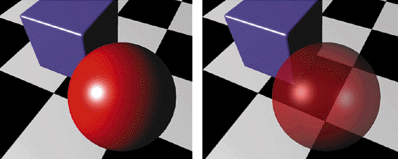
\includegraphics[width=320px]{graphics/blending.png}	
	\caption{Alpha-Blending\protect\footnotemark}
	\label{fig:AlphaBlending}
\end{figure}
\footnotetext{Quelle: \url{http://common.ziffdavisinternet.com/encyclopedia_images/_ALPHACH.GIF}}



\subsection{Billboarding}

Um unsere Vorgabe der Echtzeitfähigkeit zu erfüllen benötigt es ein paar Tricks, die es erlauben die Komplexität unseres Renderers zu minimieren, gleichzeitig jedoch darf der Zuschauer diese Manipulation nicht bemerken.
Eine beliebte Technik hierfür ist das Billboarding. Die Idee des Billboardings basiert darauf, komplexe geometrische 3D-Objekte auf ein zweidimensionales Rechteck das sogenannte Billboard runterzubrechen. 
Bei dem Billboard handelt es sich meist um ein vorher berechnetes Bild von dem ursprünglich darzustellenden 3D-Objekts.
Anschließend wird dieses Billboard zur Kamera ausgerichtet. Durch den zusätzlichen Einsatz von Blending überlappen diese 2D Objekte Objekte dann und erzeugen somit einen 3D-Effekt. Dem Zuschauer fällt es somit sehr schwer zu erkennen, das es sich bei dem gezeigten Objekt um eine zweidimensionale Kopie des 3D-Objektes handelt.
Diese Technik wird hauptsächlich dazu verwendet die benötigten Rechenoperationen für Objekte welche in der Ferne liegen zu minimieren. 
Kommt die Kamera dem tatsächlichen Objekten sehr nahe, wird meist mittels einer Interpolation zwischen dem Billboard und dem tatsächlichen 3D-Objekt umgeschaltet.
\end{Spacing}
\newpage
\clearpage
%% End Of Doc